% \Huge

\section{Cosmological Context}

Cosmology has seen many advances in the last few decades. Piece by piece we are uncovering the history of the universe and it's components. We now know that our galaxy is just one in trillions (\cite{2016ApJ...830...83C}), and part of a rapidly expanding universe. 

Our two main observational tools today are the Cosmic Microwave Background (CMB) and Galaxy Surveys. From the CMB we learn about the primordial universe, and Galaxy Surveys uncover the nature and structure of the Universe at late times. Each of them will be discussed in the next two sections.

Despite a wealth of knowledge, the nature of the two most important components of the Universe still eludes us. Dark Matter and Dark Energy account for about $95\%$ of the matter-energy budget of the universe (e.g. \cite{2016A&A...594A..13P}). 

There are also other gaps in our knowledge. Most of them are either related to the very early universe (before the CMB was emitted) or to the evolution of the Universe between recombination and the first galaxies being formed. In this project we will investigate the second gap.

\section{The Cosmic Microwave Background}

The Cosmic Microwave Background is our main observational tool for studying the early universe. It is the first light emitted in the Universe after recombination, and it encodes plenty of useful information. The CMB is the most perfect black body ever observed (\cite{1999dpf..conf.....W}). Its existence is already a strong proof in support of the Big Bang model. On the other hand, the anisotropies found in the CMB strongly support both the $\Lambda CDM$ paradigm and Inflation.

\begin{figure}
    \centering
    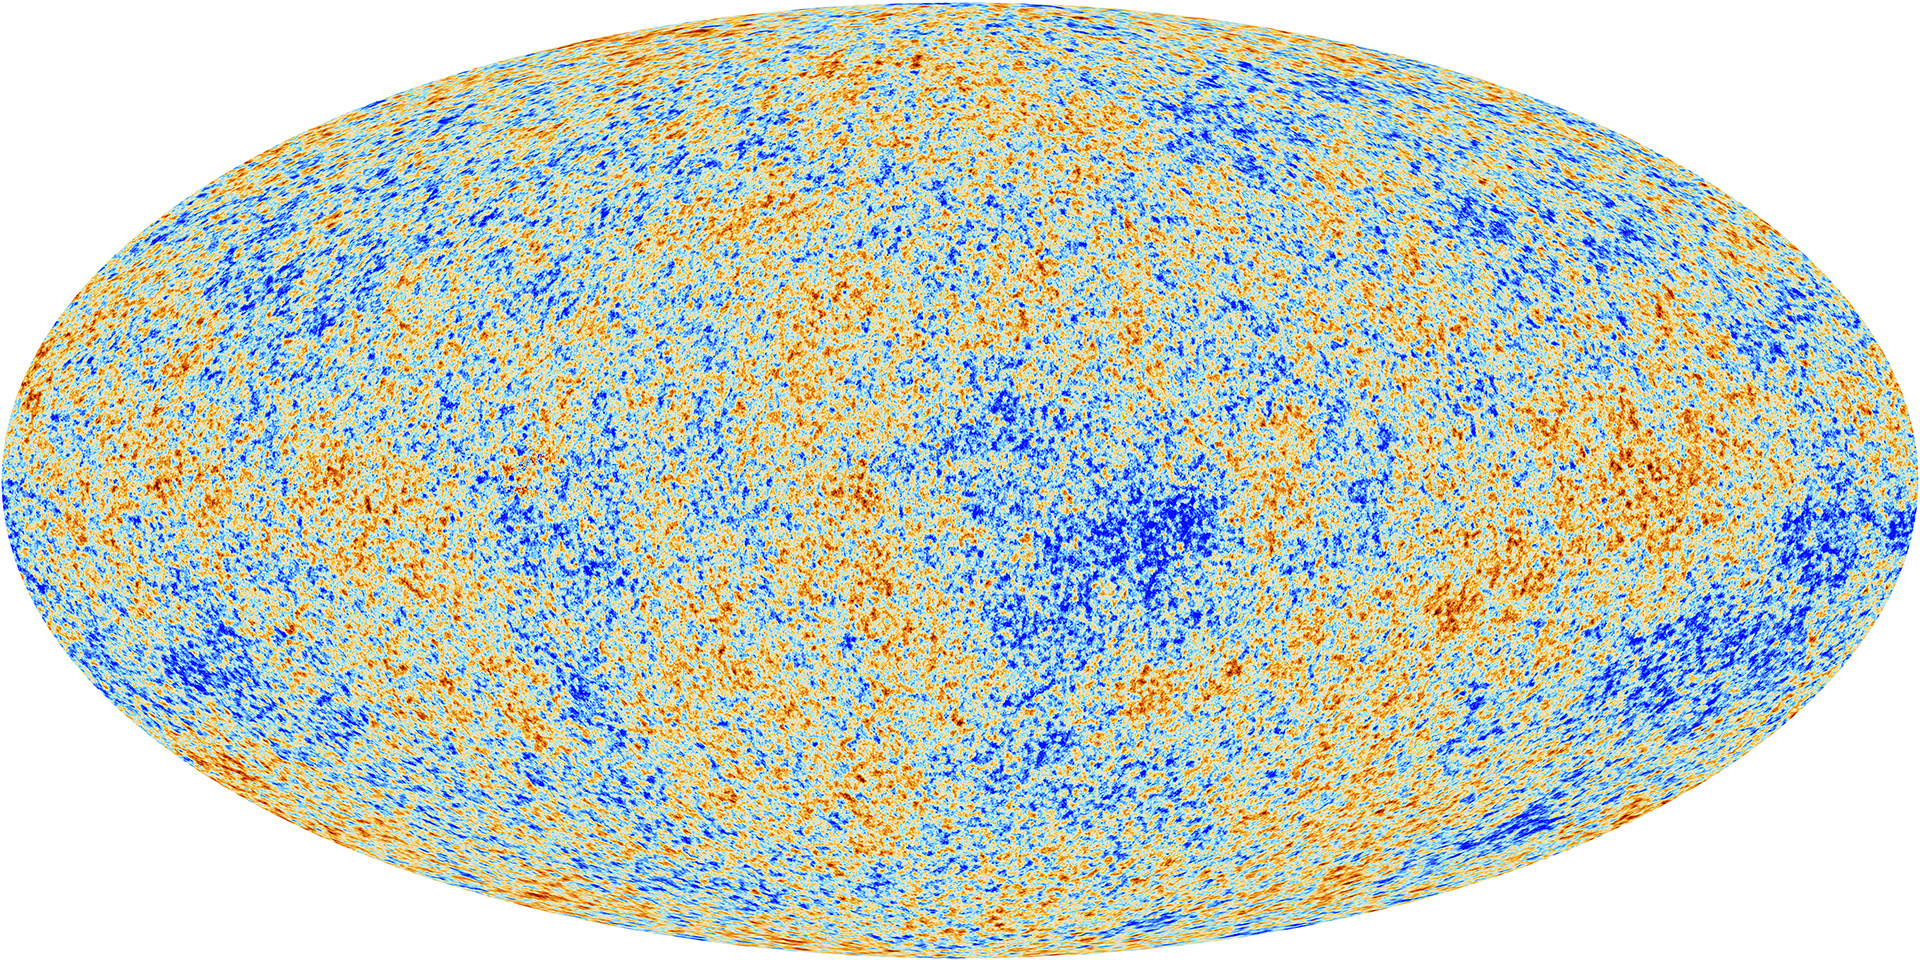
\includegraphics[width=0.9\columnwidth]{images/misc/Planck_CMB.jpg}%
    
    \caption{
    Map of the Cosmic Microwave Background aquired by the Planck Space Telescope (ref). 
    }
    
    \label{fig:1}
\end{figure}


\section{Large Scale Structure and Galaxy Surveys}

\todo[inline]{Introduce the Structure of the Universe today and the tools used to study it.}

\todo[inline]{Talk about the detection of the BAO in the galaxy distribution and its smearing due to collapse.}

\begin{figure}
    \centering
    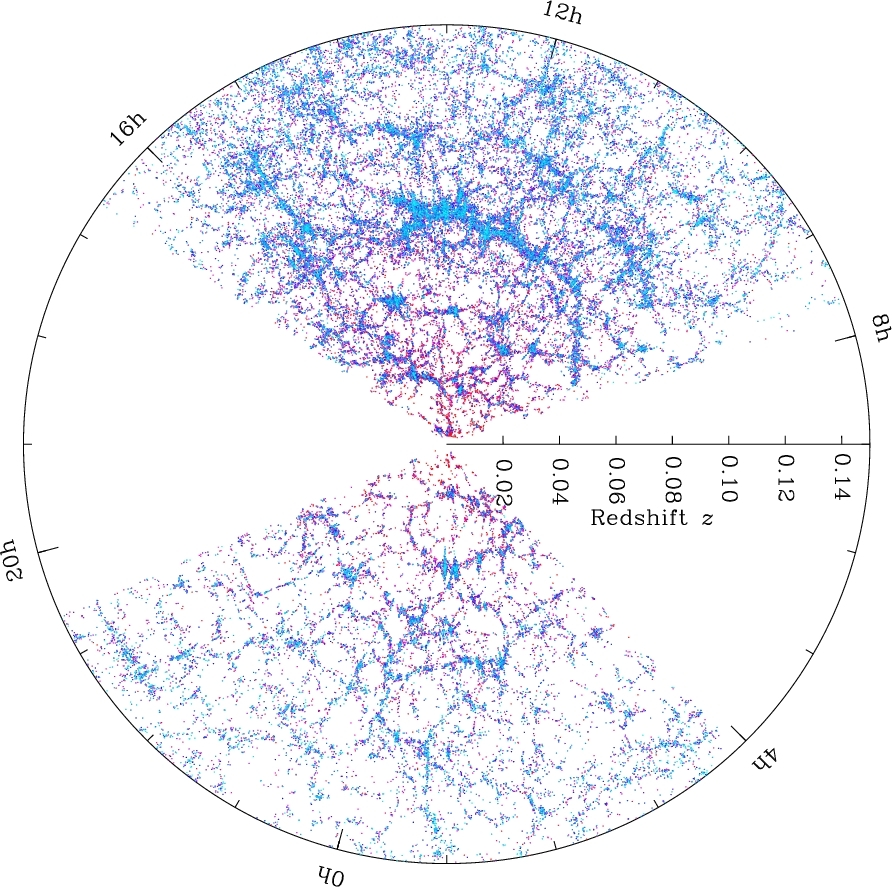
\includegraphics[width=0.9\columnwidth]{images/misc/orangepie.jpg}%
    
    \caption{
    Galaxy map from the Sloan Digital Sky Survey.
    }
    
    \label{fig:2}
\end{figure}


\section{The Missing Link (Reconstruction)}

\todo[inline]{Motivate our desire to link the two and talk about the problems we have (Dark Ages)}

\todo[inline]{Motivate the desire to reconstruct the BAO feature}
